\documentclass[12pt]{article}

\usepackage[margin=1in, left=0.6in, right=0.6in]{geometry}
\usepackage{fancyhdr}	% header
\usepackage{hyperref} % links

\usepackage{amsmath,amsthm,amssymb}	%math stuff
\usepackage{graphicx} \graphicspath{ {./images/} }
\usepackage{setspace} % increase line spacing
\usepackage{tabularx} % long tables
\usepackage{enumitem} % labelling itmes
\usepackage{color, soul}
\usepackage{lmodern} % bolding \texttt{}
\usepackage[T1]{fontenc} % for {} in \texttt{}
\usepackage{listings}
\usepackage[table]{xcolor}
\usepackage[edges]{forest}
\usepackage{xfrac} % slanted fractions
% \usepackage{array}
% \usepackage{booktabs}
% \usepackage{siunitx}
% \usepackage{alltt}

\definecolor{dkgreen}{rgb}{0,0.6,0}
\definecolor{gray}{rgb}{0.5,0.5,0.5}
\definecolor{mauve}{rgb}{0.58,0,0.82}
\definecolor{backcolour}{rgb}{0.95,0.95,0.92}

\setlength{\parindent}{0pt}

\pagestyle{fancy}
\fancyhead[LO,L]{CSCC37 A3}
\fancyhead[CO,C]{Stephen Guo}
\fancyhead[RO,R]{1006313231}
\fancyfoot[LO,L]{}
\fancyfoot[CO,C]{\thepage}
\fancyfoot[RO,R]{}

\newcommand{\N}{\mathbb{N}}
\newcommand{\R}{\mathbb{R}}
\newcommand{\Rplus}{\mathbb{R}^{+}}
\newcommand{\bigbracket}[1]{\big(#1\big)}
\newcommand{\Bigbracket}[1]{\Big(#1\Big)}
\newcommand{\floorSurround}[1]{\left\lfloor#1\right\rfloor}
\newcommand{\ceilingSurround}[1]{\left\lceil#1\right\rceil}
\newcommand{\code}[1]{{\ttfamily \fontseries{b}\selectfont #1}}
\definecolor{codegray}{gray}{0.9}
\def \calO {\mathcal{O}}
\newcommand{\bigO}[1]{\ensuremath{\calO(#1)}}
\renewcommand{\qed}{\hfill$\blacksquare$}
\newenvironment{proofindent}{\vspace*{2mm}\hfill\begin{minipage}{\dimexpr\textwidth-10mm}}{\end{minipage}}

\everymath{\displaystyle}

\begin{document}
%----------------------------------------------------------------------------------
%                              Table of Contents
%----------------------------------------------------------------------------------
\begin{center}
    \hypertarget{toc}{\LARGE \underline{\textbf{Table of Contents}}}\\
\end{center}

{\textbf{Question 1:}}
\vspace{1mm}
\hrule
\vspace{1mm}
\hyperlink{1.1}{(a)}\\
\hyperlink{1.2}{(b)}\\
\hyperlink{1.3}{(c)}\\
\hyperlink{1.4}{(d)}\\

\textbf{Question 2:}
\vspace{1mm}
\hrule
\vspace{1mm}
\hyperlink{2.1}{(a)}\\
\hyperlink{2.2}{(b)}\\

\textbf{Question 3:}
\vspace{1mm}
\hrule
\vspace{1mm}
\hyperlink{3.1}{(a)}\\
\hyperlink{3.2}{(b)}\\
\hyperlink{3.3}{(c)}\\

\hyperlink{4}{\textbf{Question 4:}}
\vspace{1mm}
\hrule
\vspace{1mm} \leavevmode \\

{\textbf{Question 5:}}
\vspace{1mm}
\hrule
\vspace{1mm}
\hyperlink{5.1}{(a)}\\
\hyperlink{5.2}{(b)}\\
\hyperlink{5.3}{(c)}\\
\hyperlink{5.4}{(d)}\\

\newpage

% {\setstretch{1.5}$\begin{array}{r@{}>{\displaystyle}l}  \end{array}$}
% {
%     \setstretch{1.5}
%     $
%         \begin{array}{r@{}>{\displaystyle}l}
%              & {} \\
%              & {} \\
%              & {} \\
%              & {} \\
%              & {} \\
%         \end{array}
%     $
% }
%----------------------------------------------------------------------------------
%                                   Questions
%----------------------------------------------------------------------------------
\setstretch{1.2}
%----------------------------------------------------------------------------------
% !                                    1
%----------------------------------------------------------------------------------
\hyperlink{toc}{\LARGE\underline{\textbf{Question 1.}}}\\
~\\\hyperlink{toc}{\hypertarget{1.1}{(a)}}\\
If there is an interval $[a,\ b]$ such that
\begin{enumerate}
    \item $g(x) \in [a,\ b] \qquad \forall x\in [a,\ b]$
    \item $|g'(x)| \leq L < 1 \qquad \forall x\in [a,\ b]$
\end{enumerate}
Then $g(x)$ has a unique fixed point in $[a,\ b]$

~\\\hyperlink{toc}{\hypertarget{1.2}{(b)}}\\
Suppose 1. and 2. \\
Start with any $x_0\in [a,\ b]$ and iterate\\
$x_{k+1} = g(x_k) \qquad k = 1,\ 2,\ \cdots$\\

Then $x_k \in [a,\ b]$ by 1.\\

Moreover, ~
{
\setstretch{1.5}
$$
    \begin{array}{r@{}>{\displaystyle}l}
        x_{k+1} - x_{k}
         & {}= g(x_{k}) - x_{k-1}          \\
         & {}= g'(\eta_k)(x_{k+1} - x_{k}) \\
    \end{array}
$$
\begin{center}
    for some $\eta_k \in [x_{k-1},\ x_k] \subset [a,\ b] \qquad$ (condition 2)
\end{center}
}

So
$$
    \begin{array}{r@{}>{\displaystyle}ll}
        x_{k+1} - x_{k}
         & {}\leq L |x_{k} - x_{k-1}|     & \\
         & {}\leq L^2 |x_{k-1} - x_{k-2}| & \\
         & {}\leq \hspace*{15mm}\vdots    & \\
         & {}\leq L^{k-1} |x_{2} - x_{1}| & \\
         & {}\leq L^k |x_{1} - x_{0}|     & \\
    \end{array}
$$
$L_k$ approaches 0 as $k$ appraoches $\infty$. So $|x_{1} - x_{0}|$ approaches 0 as well\\
$\therefore x_k$ converges to some point $\widetilde{x}\in [a,\ b]$\\

\newpage\hyperlink{toc}{\hypertarget{1.3}{(c)}}\\
WTS: $g(\widetilde{x}) = \widetilde{x}$\\
This is equivalent as setting $f(x) = g(x) - x$ and showing $\widetilde{x}$ is a root of $f(x)$\\

{
\setstretch{1.5}
$
    \begin{array}{r@{}>{\displaystyle}ll}
        f(x_{k+1})
         & {}= g(x_{k+1}) - x_{k+1}                                                       & [\text{by definition}]                                \\
         & {}= g(x_{k+1}) - g(x_{k})                                                      & [\text{since $x_{k+1} = g(x_k)$}]                     \\
         & {}= g^\prime(\eta) (x_{k+1} - x_k) \text{ for some $\eta \in [x_{k+1},\ x_k]$} & [\text{since $f(x)$ is differentiable by assumption,} \\
         & {}                                                                             & \text{\qquad we use MVT}]                             \\
    \end{array}
$
}\\
Taking the limit of both sides...\\
{
\setstretch{1.5}
$
    \begin{array}{r@{}>{\displaystyle}ll}
        f(\widetilde{x})
         & {}= \lim_{k->\infty} f\left(x_{k+1}\right)                                                      & [x_k \text{ converges to } \widetilde{x}]       \\
         & {}= \lim_{k->\infty} g^\prime(\eta) (x_{k+1} - x_k) \text{ for some $\eta \in [x_{k+1},\ x_k]$} & [\text{limit both sides}]                       \\
         & {}= g^\prime(\eta) \lim_{k->\infty} (x_{k+1} - x_k)                                             & [g^\prime(\eta) \text{ does not depend on $x$}] \\
         & {}= g^\prime(\eta) \lim_{k->\infty} (\widetilde{x} - \widetilde{x})                             & [x_k \text{ converges to } \widetilde{x}]       \\
         & {}= g^\prime(\eta) \lim_{k->\infty} 0                                                           & [\text{arithmetic}]                             \\
         & {}= 0                                                                                           & [\text{$g^\prime(\eta)$ is not infinite}]       \\
    \end{array}
$
}\\

Since $\widetilde{x}$ is a root for $f(x)$\\
$\therefore \widetilde{x}$ is a fixed point.

\newpage\hyperlink{toc}{\hypertarget{1.4}{(d)}}\\
Suppose $\widetilde{x_1},\ \widetilde{x_2}$ are fixed points of $g(x)$\\

WTS: $\widetilde{x_1} = \widetilde{x_2}$\\

{
\setstretch{1.5}
$
    \begin{array}{r@{}>{\displaystyle}ll}
        \widetilde{x_1} - \widetilde{x_2}
         & {}= g(\widetilde{x_1}) - g(\widetilde{x_2})                                                                            & [\text{since $g(x) = x$}] \\
         & {}= g^\prime(\eta) (\widetilde{x_1} - \widetilde{x_2}) \text{ for some $\eta \in [\widetilde{x_1},\ \widetilde{x_2}]$} & [\text{by MVT}]           \\
    \end{array}
$
}\\

{
Taking the absolute values of both sides:\\
\setstretch{1.5}
$
    \begin{array}{r@{}>{\displaystyle}ll}
        |\widetilde{x_1} - \widetilde{x_2}|
         & {}= |g^\prime(\eta) (\widetilde{x_1} - \widetilde{x_2})|          & [\text{absolute value both sides}]       \\
         & {}= \big|g^\prime(\eta)\big|\ |\widetilde{x_1} - \widetilde{x_2}| & [\text{splitting up the absolute value}] \\
    \end{array}
$
}\\

% ~\\\\
% {
% \setstretch{1.5}
% $
%     \begin{array}{rr@{}>{\displaystyle}ll}
%                             & \widetilde{x_1} - \widetilde{x_2}                                                                  & {}= g(\widetilde{x_1}) - g(\widetilde{x_2})                                                                            & [\text{since $g(x) = x$}]                                                         \\
%                             &                                                                                                    & {}= g^\prime(\eta) (\widetilde{x_1} - \widetilde{x_2}) \text{ for some $\eta \in [\widetilde{x_1},\ \widetilde{x_2}]$} & [\text{by MVT}]                                                                   \\

%         \Longleftrightarrow & |\widetilde{x_1} - \widetilde{x_2}|
%                             & {}= |g^\prime(\eta) (\widetilde{x_1} - \widetilde{x_2})|                                           & [\text{absolute value both sides}]                                                                                                                                                                         \\
%                             &                                                                                                    & {}= \big|g^\prime(\eta)\big|\ |\widetilde{x_1} - \widetilde{x_2}|                                                      & [\text{splitting up the absolute value}]                                          \\


%         \Longleftrightarrow & |\widetilde{x_1} - \widetilde{x_2}| - \big|g^\prime(\eta)\big| |\widetilde{x_1} - \widetilde{x_2}| & {}= 0                                                                                                                  & [\text{subtracting both sides}]                                                   \\
%         \Longleftrightarrow & \big(1 - |g^\prime(\eta)|\big) |\widetilde{x_1} - \widetilde{x_2}|                                 & {}= 0                                                                                                                  & [\text{factoring}]                                                                \\
%         \Longleftrightarrow & |\widetilde{x_1} - \widetilde{x_2}|                                                                & {}= 0                                                                                                                  & [\text{dividing both sides since $\big(1 - |g^\prime(\eta)|\big)$ is never zero}] \\
%         \Longleftrightarrow & \widetilde{x_1}                                                                                    & {}= \widetilde{x_2}                                                                                                    & [\text{trivial}]                                                                  \\
%     \end{array}
% $
% }
% ~\\\\

Subtracting both sides:\\
{
\setstretch{1.5}
$
    \begin{array}{rr@{}>{\displaystyle}ll}
                            & |\widetilde{x_1} - \widetilde{x_2}| - \big|g^\prime(\eta)\big| |\widetilde{x_1} - \widetilde{x_2}| & {}= 0               & [\text{subtracting both sides}]                                                   \\
        \Longleftrightarrow & \big(1 - |g^\prime(\eta)|\big) |\widetilde{x_1} - \widetilde{x_2}|                                 & {}= 0               & [\text{factoring}]                                                                \\
        \Longleftrightarrow & |\widetilde{x_1} - \widetilde{x_2}|                                                                & {}= 0               & [\text{dividing both sides since $\big(1 - |g^\prime(\eta)|\big)$ is never zero}] \\
        \Longleftrightarrow & \widetilde{x_1}                                                                                    & {}= \widetilde{x_2} & [\text{trivial}]                                                                  \\
    \end{array}
$
}\\

as wanted. \qed

\newpage
%----------------------------------------------------------------------------------
% !                                    2
%----------------------------------------------------------------------------------
\hyperlink{toc}{\LARGE \underline{\textbf{Question 2.}}}\\
~\\\hyperlink{toc}{\hypertarget{2.1}{(a)}}\\
$f$ has one root. This is calculated by setting
$f(x) = 1-\frac{1}{2x} = 0 \qquad\Longrightarrow\qquad x = \frac{1}{2}$\\

$g\left(\frac{1}{2}\right) = 2\left(\frac{1}{2}\right)\left(1-\frac{1}{2}\right) = \frac{1}{2}$\\
$\Longrightarrow g\left(\frac{1}{2}\right) = \frac{1}{2}$\\
$\therefore \frac{1}{2}$ is a fixed point\\

To check if there are any other fixed points, solve\\
{
\setstretch{1.5}
$
    \begin{array}{rr@{}>{\displaystyle}l}
                            & 2x(1-x)   & {}= x               \\
        \Longleftrightarrow & x - 2x^2  & {}= 0               \\
        \Longleftrightarrow & x(1 - 2x) & {}= 0               \\
        \Longleftrightarrow & x         & {}= 0,\ \frac{1}{2} \\
                            &           & {}                  \\
    \end{array}
$
}\\
$\therefore 0$ is a fixed point which isn't a root of $f(x)$

\newpage\hyperlink{toc}{\hypertarget{2.2}{(b)}}\\
We can find the number of fixed points of $g(x)$ by using the Fixed Point Theorem\\
$g^\prime(x) {}= 2-4x$\\
{
\setstretch{1.5}
$
    \begin{array}{rr@{}>{\displaystyle}ll}
                            & |g^\prime(x)| & {}< 1                                        & [\text{by FPT}]          \\
        \Longleftrightarrow & |2-4x|        & {}< 1                                        & [\text{substituting}]    \\
        \Longleftrightarrow & \left\{
        \begin{aligned}
            \ 2-4x   & \hspace*{13mm} \text{if }  2-4x > 0   \\
            \ 4x - 2 & \hspace*{13mm} \text{if } 2-4x \leq 0 \\
        \end{aligned}
        \right.             & {}<  1        & [\text{change absolute values to piecewise}]                            \\
        \Longleftrightarrow & \left\{
        \begin{aligned}
            \ 2-4x   & \hspace*{13mm} \text{if }  x < \frac{1}{2}   \\
            \ 4x - 2 & \hspace*{13mm} \text{if } x \geq \frac{1}{2} \\
        \end{aligned}
        \right.             & {}< 1         & [\text{simplifying}]                                                    \\
        \Longleftrightarrow & x             & {}\in \left[\frac{1}{4},\ \frac{3}{4}\right] & [\text{solving for $x$}] \\
    \end{array}
$
}\\

So condition 2 is satisfied with that range.\\

For condition 1, we can plot the graph of $g(x)$\\
\begin{center}
    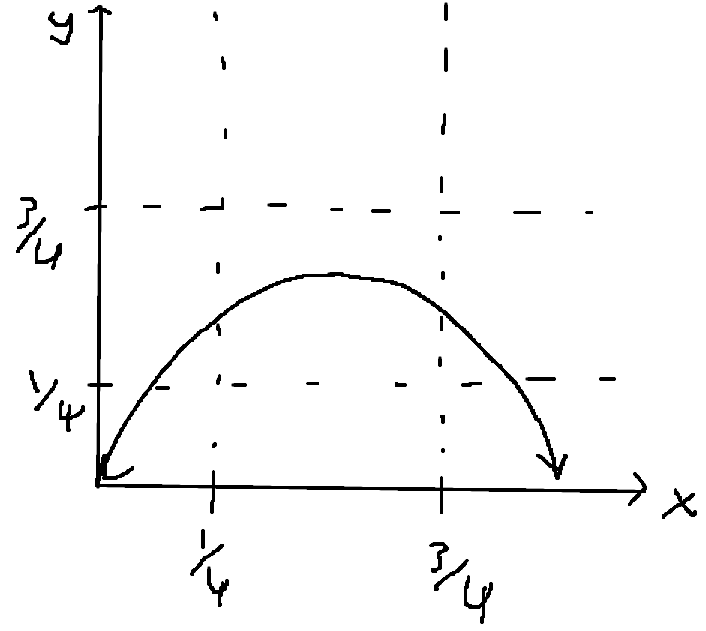
\includegraphics[width=10cm]{cscc37-a3-2b.png}\\
\end{center}
We can see that $g(x) \in \bigl[\frac{1}{4},\ \frac{3}{4}\bigr]\qquad \forall x \in \bigl[\frac{1}{4},\ \frac{3}{4}\bigr]$\\
$\therefore$ condition 1 is satisfied.\\

$\therefore$ the range $\bigl[\frac{1}{4},\ \frac{3}{4}\bigr]$ guarantees convergence.

\newpage
%----------------------------------------------------------------------------------
% !                                    3
%----------------------------------------------------------------------------------
\hyperlink{toc}{{\LARGE \underline{\textbf{Question 3.}}}}\\
~\\\hyperlink{toc}{\hypertarget{3.1}{(a)}}\\
Let $f(x) = x + \ln(x) = 0$\\
Then $x = -\ln(x)$\\
$\Longrightarrow (1)$ is a valid formula\\

{
\setstretch{1.5}
$
    \begin{array}{rr@{}>{\displaystyle}l}
                            & x      & {}= -\ln(x) \\
        \Longleftrightarrow & \ln(x) & {}= -x      \\
        \Longleftrightarrow & x      & {}=e^{-x}   \\
    \end{array}
$
}\\

$\Longrightarrow (2)$ is a valid formula\\

{
\setstretch{1.5}
$
    \begin{array}{rr@{}>{\displaystyle}l}
                            & x  & {}= e^{-x}               \\
        \Longleftrightarrow & 2x & {}= x + e^{-x}           \\
        \Longleftrightarrow & x  & {}= \frac{x + e^{-x}}{2} \\
    \end{array}
$
}\\

$\Longrightarrow (3)$ is a valid formula\\

% {
%     \setstretch{1.5}
%     $
%         \begin{array}{rr@{}>{\displaystyle}l}
%              \Longleftrightarrow & {}= \\
%              \Longleftrightarrow & {}= \\
%              \Longleftrightarrow & {}= \\
%              \Longleftrightarrow & {}= \\
%              \Longleftrightarrow & {}= \\
%         \end{array}
%     $
% }

~\\\hyperlink{toc}{\hypertarget{3.2}{(b)}}\\
{
\setstretch{3}
$
    \begin{array}{r@{}>{\displaystyle}l@{}>{\displaystyle}l}
        (1)\qquad g^\prime\left(\frac{1}{2}\right) & {}= -\frac{1}{\frac{1}{2}}          & {}= -2         \\
        (2)\qquad g^\prime\left(\frac{1}{2}\right) & {}= -e^{-\frac{1}{2}}               & {}\approx -0.6 \\
        (3)\qquad g^\prime\left(\frac{1}{2}\right) & {}= \frac{1}{2}(1-e^{-\frac{1}{2}}) & {}\approx 0.2  \\
    \end{array}
$
}\\

$\therefore (3)$ should be used since $g^\prime\left(\frac{1}{2}\right)$ is closest to 0.\\

\newpage\hyperlink{toc}{\hypertarget{3.3}{(c)}}\\

Using newtons method:\\
\hspace*{1mm}$g(x) = x - \frac{f(x)}{f^\prime(x)}$\\
$g^\prime(\widetilde{x}) = \frac{f(\widetilde{x}) f^{\prime\prime}(\widetilde{x})}{f^\prime(\widetilde{x})^2}$\\\\

{
\setstretch{1.5}
$
    \begin{array}{r@{}>{\displaystyle}l}
        f(x)                & {}= x + \ln(x)      \\
        f^{\prime}(x)       & {}= 1 + \frac{1}{x} \\
        f^{\prime\prime}(x) & {}= -\frac{1}{x^2}  \\
    \end{array}
$
}\\\\

{
\setstretch{1.5}
$
    \begin{array}{r@{}>{\displaystyle}l}
        g(x) & {}= x - \frac{1-\ln(x)}{1 + \frac{1}{x}}                                                   \\
             & {}= x - \frac{x-x\ln(x)}{x+1}                                                              \\
             & {}= \frac{x^2 + x\ln(x)}{x+1}                                                              \\
        \\
        g^\prime(x) = \frac{f(\widetilde{x}) f^{\prime\prime}(\widetilde{x})}{f^\prime(\widetilde{x})^2}
             & {}= \frac{\big(x + \ln(x)\big)\left(-\frac{1}{x^2}\right)}{\left(1 + \frac{1}{x}\right)^2} \\
             & {}= -\frac{x + \ln(x)}{(x+1)^2}                                                            \\
    \end{array}
$
}\\

$g^\prime\left(\frac{1}{2}\right) \approx 0.09$\\
$\therefore g(x) = \frac{x^2 + x\ln(x)}{x+1}$ is a better formula.
\newpage
%----------------------------------------------------------------------------------
% !                                    4
%----------------------------------------------------------------------------------
\hyperlink{toc}{\hypertarget{4}{\LARGE \underline{\textbf{Question 4.}}}}\\

% $x_{k+1} = 2x_k - {x_k}^2y$\\
% $x_{k+1} = x_k - ({x_k}^2y + x_k)$\\

{
\setstretch{1.5}
$
    \begin{array}{rr@{}>{\displaystyle}l}
                            & x_{k+1} & {}= 2x_k - {x_k}^2y        \\
        \Longleftrightarrow & x_{k+1} & {}= x_k - ({x_k}^2y - x_k) \\
    \end{array}
$
}\\

So $\frac{f(x)}{f^\prime(x)} = {x_k}^2y - x_k$\\

Since we are using Newton's method, we can assume it converges. Which means\\
$\frac{f(x)}{f^\prime(x)} = {x_k}^2y - x_k = 0$\\
{
\setstretch{2.5}
$
    \begin{array}{rr@{}>{\displaystyle}l}
                            &\frac{f(x)}{f^\prime(x)}  = {x_k}^2y - x_k & {}= 0\\
        \Longleftrightarrow &  x_k({x_k}y - 1)& {}= 0\\
    \end{array}
$
}\\

So we have $x_k = 0,\ \frac{1}{y}$\\

% {
% \setstretch{2.5}
% $
%     \begin{array}{rr@{}>{\displaystyle}l}
%                             & \frac{f(x)}{f^\prime(x)} & {}= {x_k}^2y - x_k         \\
%         \Longleftrightarrow & \frac{f^\prime(x)}{f(x)} & {}= \frac{1}{{x_k}^2y - x_k}        \\
%         \Longleftrightarrow & \int\frac{f^\prime(x)}{f(x)} \text{dx}& {}= \int\frac{1}{{x_k}^2y - x_k} \text{dx}        \\
%         \Longleftrightarrow & \ln\bigl(f(x)\bigr)& {}= \ln(xy+1) - \ln(x)                         \\
%         \Longleftrightarrow & f(x)& {}= \frac{xy-1}{x}                        \\
%     \end{array}
% $
% }\\

$\therefore$ this fixed-point iteration is used to estimate $\frac{1}{y}$

\newpage
%----------------------------------------------------------------------------------
% !                                    5
%----------------------------------------------------------------------------------
\hyperlink{toc}{{\LARGE \underline{\textbf{Question 5.}}}}\\
~\\\hyperlink{toc}{\hypertarget{5.1}{(a)}}\\
Suppose we find a root $\alpha$ such that $f(\alpha) = 0$.\\

{
\setstretch{1.5}
$
    \begin{array}{r@{}>{\displaystyle}l}
        g(\alpha) & {}= \alpha - \frac{f(\alpha)^2}{f\big(\alpha + f(\alpha)\big)-f(\alpha)} \\
                  & {}= \alpha - \frac{0^2}{f\big(\alpha + 0\big)-0}                         \\
                  & {}= \alpha - \frac{0}{0}                                                 \\
        %  & {}= \\
    \end{array}
$
}\\

all roots of $f(x)$ makes $g(x)$ diverge.
However, taking the limit as $x \rightarrow \alpha$ will make $g(\alpha)$ converge to 0\\
$\therefore$  roots of $f(x)$ are not fixed points of $g(x)$\\

There are no other fixed point of $g(x)$. Since if the numerator vanishes, then so will the denominator
which will make $g(x)$ diverge.

~\\\hyperlink{toc}{\hypertarget{5.2}{(b)}}\\
{
\setstretch{3}
$
    \begin{array}{r@{}>{\displaystyle}ll}
        g(x) & {}= x - \frac{f(x)}{f^\prime(x)}                                                   & [\text{by Newton's Method}]                 \\
             & {}= x - \frac{f(x)}{\displaystyle\lim_{h \rightarrow 0}\frac{f(x+h) - f(x)}{h}}    & [\text{by derivative limit definition}]     \\
             & {}= x - \frac{f(x)}{\displaystyle\lim_{h \rightarrow f(x)}\frac{f(x+h) - f(x)}{h}} & [\text{since we're looking for $f(x) = 0$}] \\
             & {}= x - \frac{f(x)}{\displaystyle\frac{f\big(x+f(x)\big) - f(x)}{f(x)}}            & [\text{plugging in f(x)}]                   \\
             & {}= x - \frac{f(x)^2}{f\big(x+f(x)\big) - f(x)}                                    & [\text{arithmetic}]                         \\
    \end{array}
$
}\\

as wanted

\newpage\hyperlink{toc}{\hypertarget{5.3}{(c)}}\\
Enough to show: $g^\prime(x) = 0$\\

$\hspace*{0.5mm}f^\prime(x) = 2x-10$\\
$f^{\prime\prime}(x) = 2$\\

\textbf{Newtons method}:\\
{
\setstretch{2.5}
$
    \begin{array}{r@{}>{\displaystyle}l}
        g^\prime(x) & {}= \frac{f(x) f^{\prime\prime}(x)}{f^\prime(x)^2} \\
                    & {}= \frac{(x^2-10x+24)(2)}{(2x-10)^2}              \\
                    & {}= \frac{2x^2-20x+48}{4x^2-40x-100}               \\
    \end{array}
$
}\\

$g^\prime(4) = 0$\\
$g^\prime(6) = 0$\\
$\therefore$ by RCT, Newton's method are quadratically convergent when $x$ is near 4 and 6.\\

\textbf{Steffensen's method}:\\
{
\setstretch{2.5}
$
    \begin{array}{r@{}>{\displaystyle}l}
        g(x) & {}= x - \frac{(x^2-10x+24)^2}{\big((x + x^2-10x+24)^2-10(x + x^2-10x+24)+24\big) - (x^2-10x+24)}            \\
             & {}= x - \frac{x^4 - 20x^3 + 148x^2 - 480x + 576}{\big((x^2-9x+24)^2-10(x^2-9x+24)+24\big) - (x^2-10x+24)}   \\
             & {}= x - \frac{x^4 - 20x^3 + 148x^2 - 480x + 576}{x^4-18x^3+129x^2-432x+576 -10x^2 + 90x + 240 - x^2+10x-24} \\
             & {}= x - \frac{x^4 - 20x^3 + 148x^2 - 480x + 576}{x^4 - 18 x^3 + 118 x^2 - 332 x + 792}                      \\
    \end{array}
$
}\\

$g^\prime(x) = 1 - {\textstyle\frac{(4 x^3 - 60 x^2 + 296 x - 480)(x^4 - 18 x^3 + 118 x^2 - 332 x + 792) + (x^4 - 20x^3 + 148x^2 - 480x + 576)(-332 + 236 x - 54 x^2 + 4 x^3)}{(x^4 - 18 x^3 + 118 x^2 - 332 x + 792)^2}}$\\

$g^\prime(4) = 0$\\
$g^\prime(6) = 0$\\
$\therefore$ by RCT, Steffensen's method are quadratically convergent when $x$ is near 4 and 6.\\

~\\\hyperlink{toc}{\hypertarget{5.4}{(d)}}\\
We don't need to compute $f^\prime(x)$. $f^\prime(x)$ may be expensive to calculate.
\end{document}